\graphicspath{{./figures}}

\section{Range}

Line-of-sight range tests were conducted. Both antennas were manually positioned during the tests, and the PQ dipole was both horizontally and vertically placed. All measurements were done at the originally designed parameters (e.g. SF 8, CR 4/6, 500 kHz) and with automatic gain control (AGC). The resulting \textit{received signal strength indicator} (RSSI), signal-to-noise (SNR) ratio, and packet reception rate (PRR i.e. percentage of non-corrupted packets received) was recorded. For the unfamiliar reader, the highest (best) theoretical RSSI is 0 dB, and the minimum SNR for SF 8 is -10 dB (note that LoRa is capable of demodulating negative signal-to-noise ratios).

Tests were done in locations around the Western Cape. These locations are described and mapped in Appendix \ref{sec:appendix_range}. The first primitive test (which is not listed) was a 300 m test on Coetzenburg field in Stellenbosch. The performance of this test was found to be low compared to subsequent tests, with an RSSI of around -92 dBm recorded. It is assumed that ground bounce was the major contributing factor to this, due to the low operating frequency of the system (around 430 MHz) and the close proximity of the antennas to the ground.

The final results are plotted as a function of distance in Figures \ref{fig:rangeRssi} and \ref{fig:rangeSnr}, with a logarithmic curve fit. All measurements were taken as an average of at least 10 consecutive samples. The packet contents were verified using a packet ID, the GPS location of the transmitter, as well as inspecting whether a CRC (Cyclic Redundancy Check) error had occurred. If any of these were incorrect, the packet was considered "missed".

\begin{figure}[!htb]
  \begin{minipage}{0.5\textwidth}
    \centering
    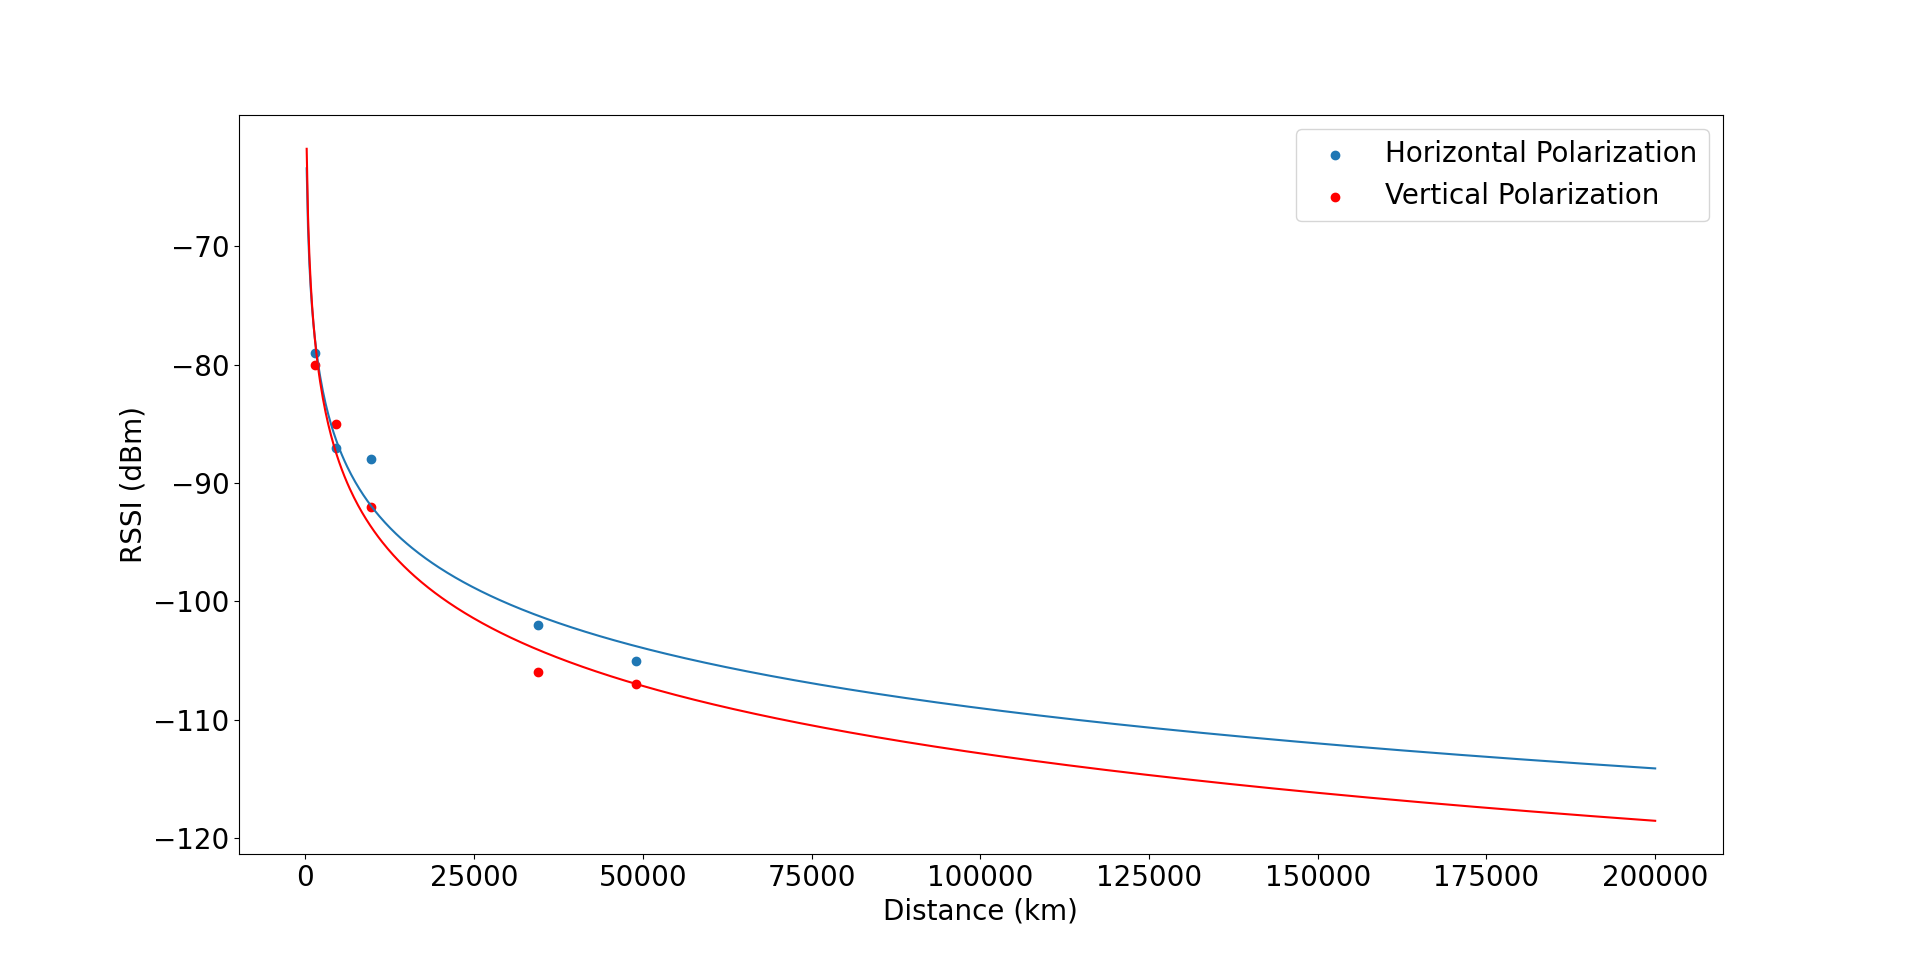
\includegraphics[width=0.99\linewidth]{rangeRssi}
    \caption{Measured RSSI vs Distance}
    \label{fig:rangeRssi}
  \end{minipage}
  \begin{minipage}{0.5\textwidth}
    \centering
    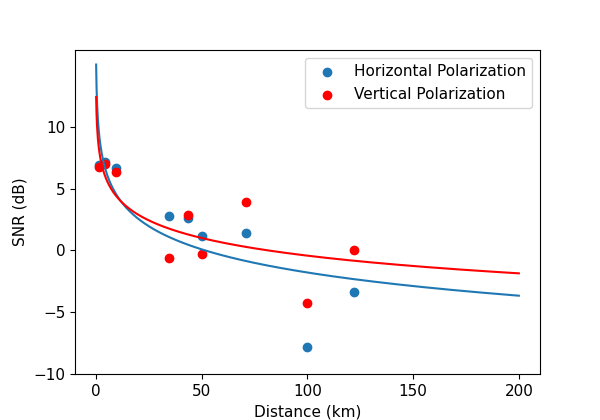
\includegraphics[width=0.99\linewidth]{rangeSnr}
    \caption{Measured SNR vs Distance}
    \label{fig:rangeSnr}
  \end{minipage}
\end{figure}

The data shows that the system successfully met the range requirement, as a reliable link was estabilished at a range of 122 km. All tests recorded a PRR of 100 \% once the system was in steady-state. The final test at 122 km recorded an RSSI of around -108 dBm for the preferred vertically polarized case. Since the receiver sensitivity is around -119 dBm, this indicates an 11 dB margin, which is slightly larger than the designed value of 10 dB. It should be noted that the 100 km should be considered an outlier - the test location on Table Mountain was chosen sub-optimally due to poor visibility caused by clouds, and it is assumed that multi-path affects lowered the signal strength. It should also be noted that the SNR logarithmic fit is not considered reliable, since the receiver appears to adjust the gain to keep the SNR around 7.5 dB for closer distances. However, the RSSI appears to follow a logarithmic curve as predicted by the free space path loss formulae.